In order to measure the performance of the different systems, the \textit{Equal Error Rate} metric
is chosen. As its name suggests, the \textit{EER} prioritizes in an equal manner the
\textit{False Positive Rate} and the \textit{False Negative Rate}.
This metric was used
in the previous works of the current line of investigation related to pronunciation assessment
at phone level \cite{detection_phone_level_mispronunciation_learning, main}, so the same approach
was taken in the present work.

The process for evaluating the performance of a classifier usually involves the following steps:
At first, the decision function of the classifier, which can be for example predicted probabilities
or in our case distances to the hyperplane, is computed for each instance of the test set.
Then, the obtained results are used to generate
a distribution of the instances count as function of the values
in the domain of the decision function. Finally,
in order to make class predictions a threshold is chosen and the instances with a result of the
decision function above that threshold are classified as positive, while
those with results below the threshold are classified as negative. Most classifiers
usually set a threshold by default, such as 0 in the case of Support Vector Machines that
determines a separation of
positives and negative instances according to the sign of their distance to the hyperplane.

The EER can be found by sweeping the threshold until reaching the condition that
False Positive Rate (FPR) equals False Negative Rate (FNR). FPR is computed as
the proportion of negative instances wrongly
categorized as positive: $\frac{FP}{TN+FP}$.
Analogously, FNR is computed as the proportion of positve
instances wrongly categorized as negative:
$\frac{FN}{TP+FN}$. A simple example of EER threshold is
shown in Fig. \ref{fig:eer}.

\begin{figure}[H]
  \centering
  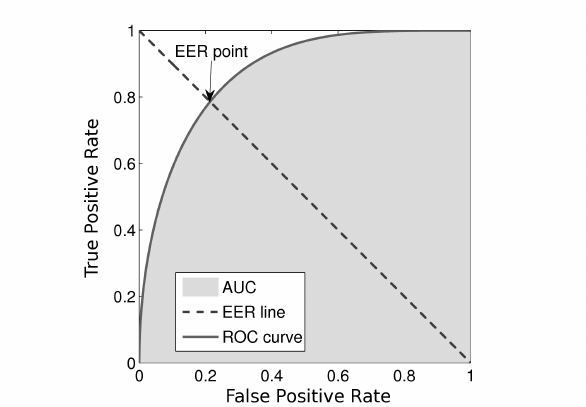
\includegraphics[width=0.8\textwidth]{files/figures/method/eer}
  \caption{An example of EER threshold with perfectly balanced classes. Both negative and positive distributions have the same size and shape.
  The threshold separates the instances in such way that FPR equals FNR.}
  \label{fig:eer}
\end{figure}
